\section{Desarrollo de un prototipo de lanzadera electromagnética}
\label{sec:prototipo}

El desarrollo del prototipo de la lanzadera electromagnética constituye una etapa crucial en la validación del modelo teórico y las diferentes simulaciones realizadas en fases previas. Esta sección se centra en el diseño y construcción de un dispositivo funcional que permita la evaluación práctica de los conceptos estudiados y la obtención de datos experimentales que respalden las predicciones teóricas.

El objetivo principal del prototipo es proporcionar una plataforma experimental (a la que se le llamará \textit{banco de pruebas}) que permita comprobar la efectividad de las configuraciones propuestas y realizar ajustes basados en observaciones empíricas. No se pretende construir una lanzadera electromagnética como la de la figura \ref{fig:prototipolanzadera}, sino más bien un prototipo modular que sea fácilmente modificable para poder probar diferentes configuraciones de bobina y alimentación. Una de las partes más importantes del prototipo ha sido la implementación de un sistema de medición capaz de registrar con exactitud la velocidad y fuerza del proyectil.

El siguiente apartado detalla los pasos específicos seguidos en el desarrollo del prototipo, desde el montaje del banco de pruebas, el diseño del circuito electrónico y la construcción de la bobina, hasta el ensamblaje del sistema completo, así como algunas de las consideraciones de diseño que los alumnos tendrán que tener en cuenta a la hora de realizar la práctica.

\begin{figure}[H]
    \centering
    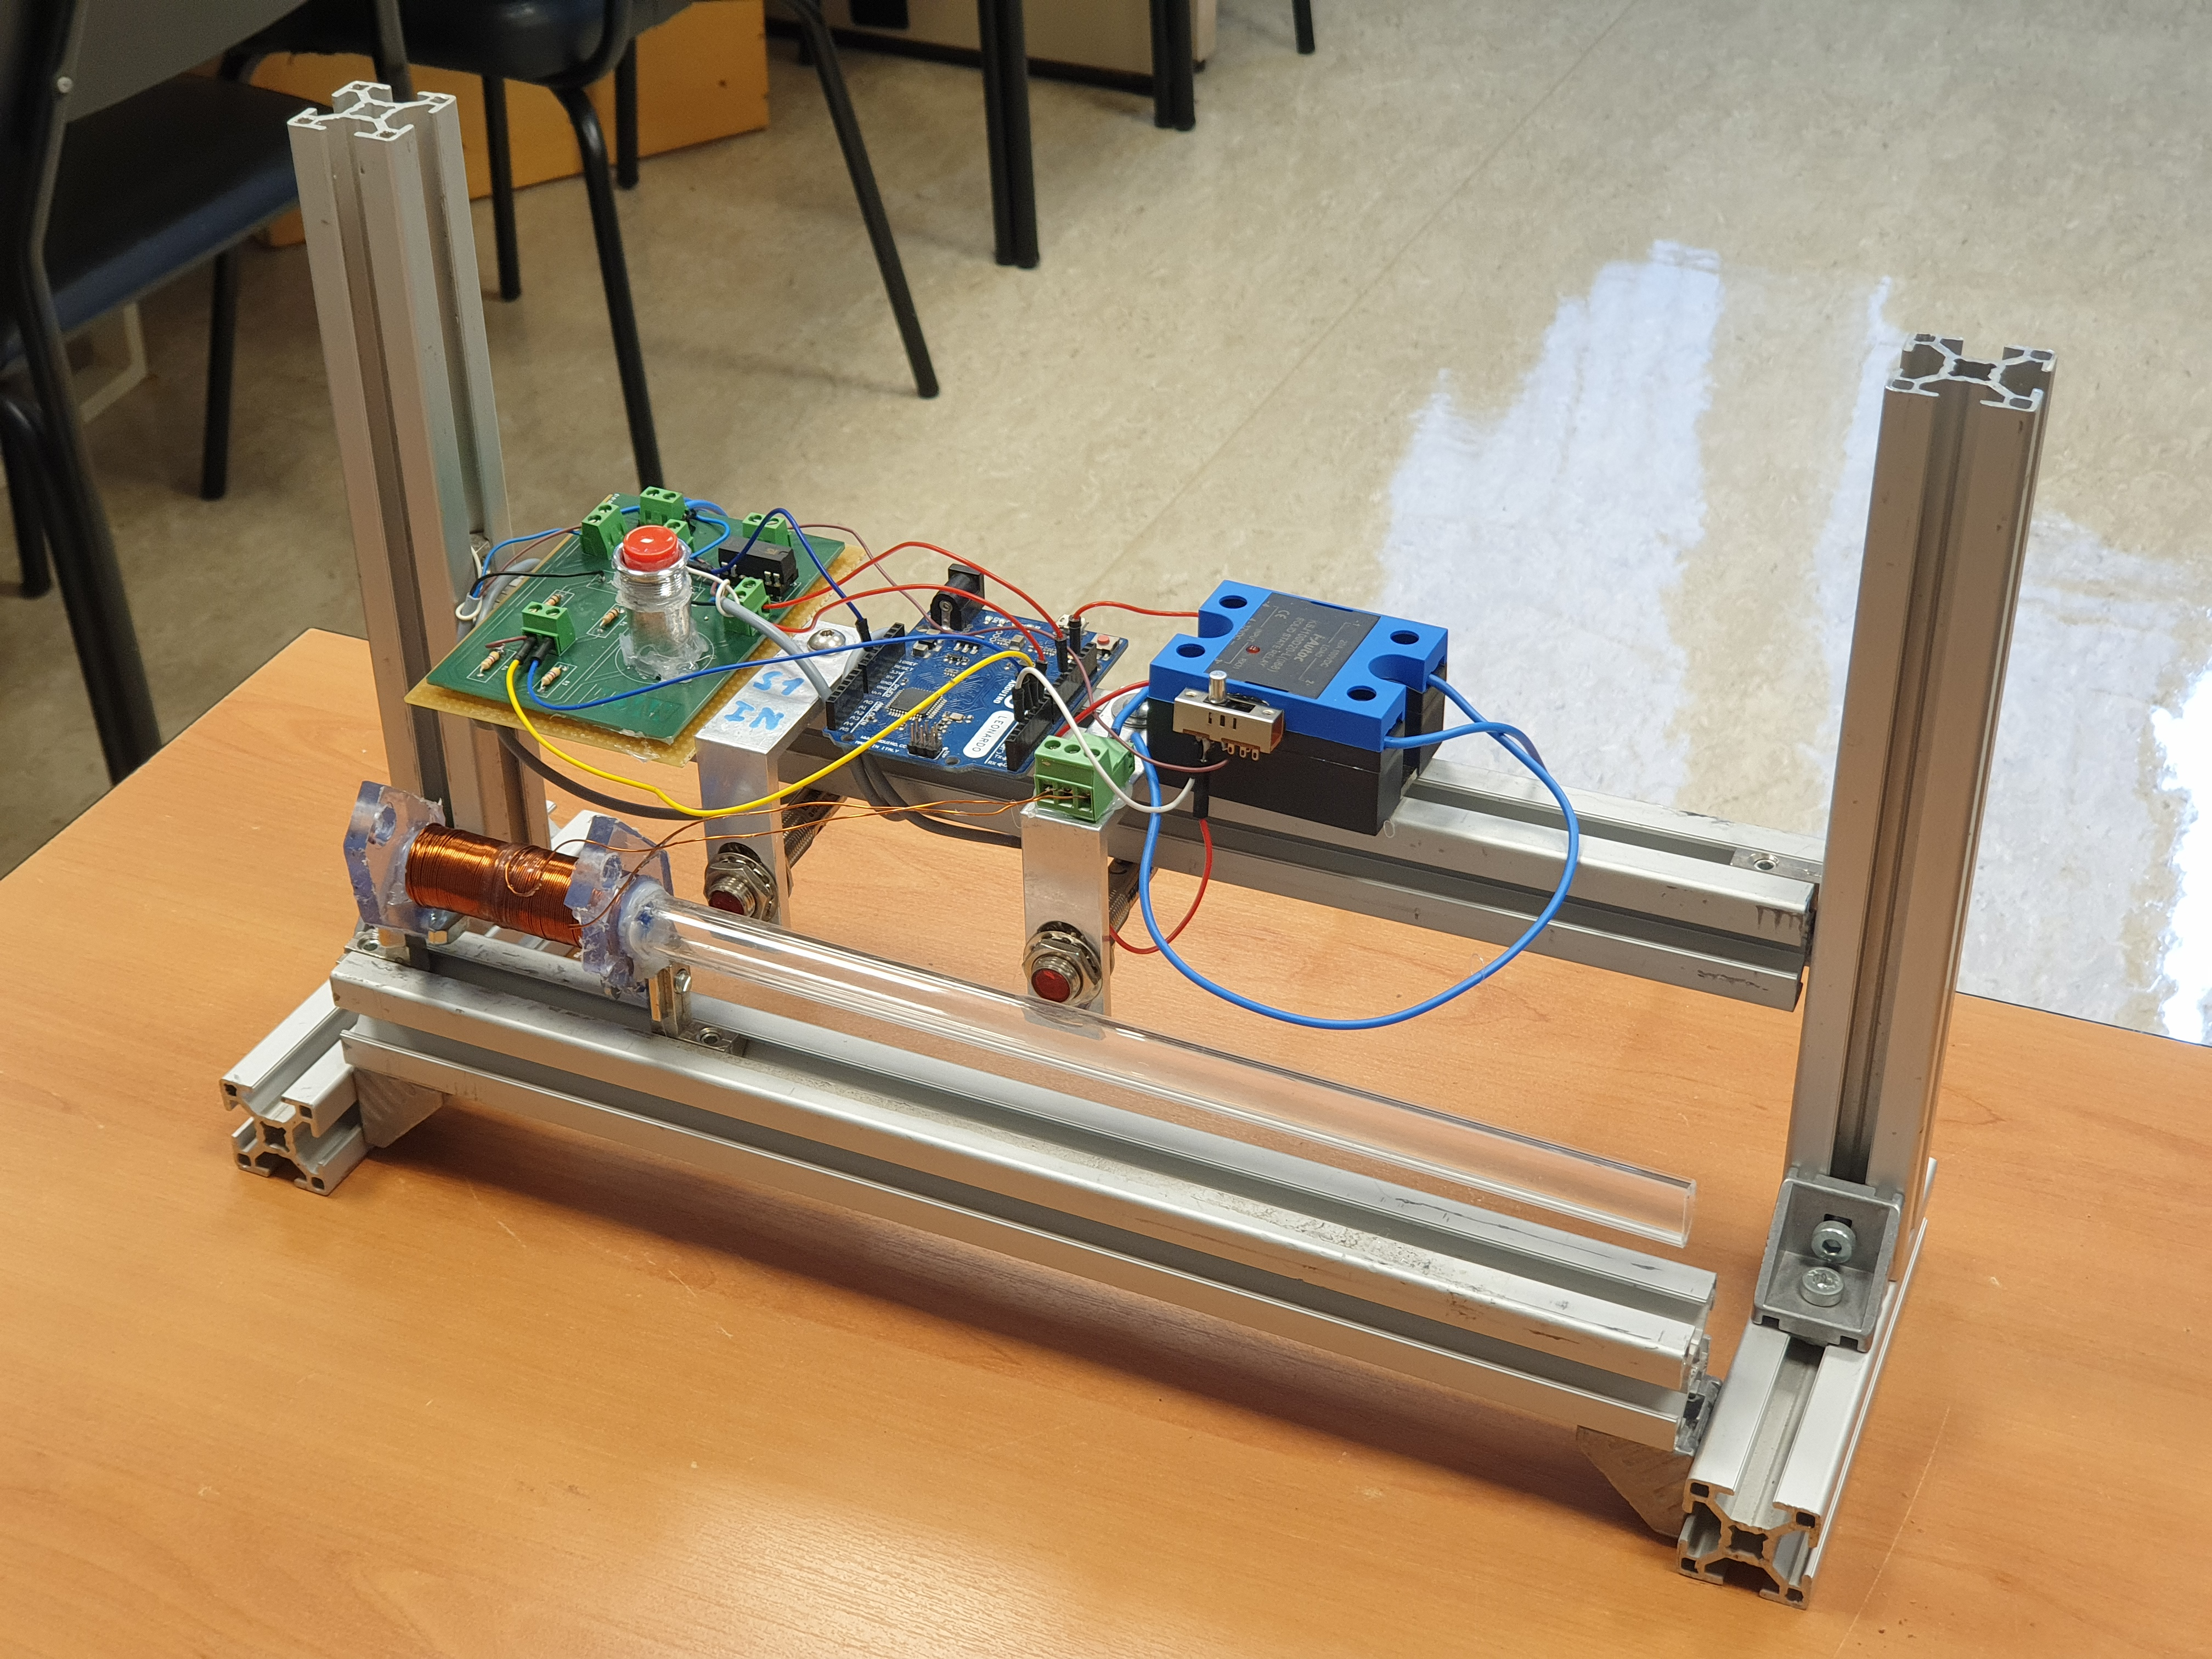
\includegraphics[width=\textwidth]{FigurasMemoria/prototipoFinal.jpg}
    \caption{Imagen del banco de pruebas definitivo.}
    \label{fig:prototipoFinal} %Para referenciar -> \ref{fig:figNum}
\end{figure}

\newpage

\subsection{Prueba inicial}

Antes de continuar con el desarrollo del prototipo, se ha realizado una prueba con un dinamómetro sobre la bobina de prueba especificada anteriormente para poder validar los resultados obtenidos en los apartados anteriores respecto a una referencia. El resultado obtenido es el siguiente:

\begin{figure}[H]
    \centering
    \includegraphics[width=9cm]{FigurasMemoria/dinamometro.jpg}
    \caption{Dato experimental de fuerza con la bobina alimentada.}
    \label{fig:dinamometro} %Para referenciar -> \ref{fig:figNum}
\end{figure}

\[F_{barra}=2~\text{N}~\forall I_{cc}=3.5~\text{A}\]

\subsection{Estructura}
\label{subsec:estructura}
Para construir una estructura estable para el banco de pruebas, se utilizaron perfiles técnicos estructurales de aluminio como el que se presenta en la siguiente figura:

\begin{figure}[H]
    \centering
    \includegraphics[width=6cm]{FigurasMemoria/perfiles.jpg}
    \caption{Perfiles de aluminio utilizados en la estructura.}
    \label{fig:perfiles} %Para referenciar -> \ref{fig:figNum}
\end{figure}

La ventaja de utilizar estos perfiles es que se puede modificar de manera muy sencilla la distribución de las diferentes partes del montaje, las cuales consisten en: dos parejas de perfiles en \textbf{T} que sirven de apoyo para el resto de la estructura, un perfil inferior que es en el que se coloca la bobina y un perfil superior que es en el que se colocan los sensores de movimiento y el circuito electrónico.

\subsection{Sensores de movimiento}
\label{subsec:sensoresmov}

Los sensores de movimiento utilizados para el proyecto tienen como objetivo proporcionar la diferencia temporal que se utilizará para el cálculo de la velocidad de salida del vástago. Los sensores que se han empleado son sensores de carácter capacitivo, lo que significa que detectan la presencia de un objeto delante de ellos por el cambio de la capacidad con la superficie del sensor. Colocando dos de estos dispositivos a una distancia conocida \textit{d} y obteniendo la diferencia temporal \(\Delta t\) de activación de la señal mediante una placa arduino conectada al sistema, es trivial calcular la velocidad del vástago según la fórmula:

\[v_{vas}=\frac{d}{\Delta t}\]

Los sensores elegidos para llevar a cabo esta tarea son los GLV12-8-200/37/40b/115, los cuales tienen el siguiente esquema de conexión:

\begin{figure}[H]
    \centering
    \includegraphics[width=10cm]{FigurasMemoria/esquemaSensor.png}
    \caption{Esquema conexiones de los sensores capacitivos.}
    \label{fig:esquemaSensor} %Para referenciar -> \ref{fig:figNum}
\end{figure}

Observando las especificaciones de este modelo detalladas en las \textit{datasheets} al final del documento, encontramos que la tensión de alimentación del sensor es de \(V_{cc}\in [10,~30]~\text{V}\), y la salida de la señal (tensión entre \textbf{SIG} y \textbf{GND}) es de \(V_{sig}=V_{cc}\). Esto es algo a tener en cuenta, pues la entrada de los puertos de arduino no puede superar los 5 V y los sensores deben ser alimentados al menos a 5 V. Montando el prototipo, se decidió que el circuito electrónico iba a estar alimentado a 15 V, por lo que será necesario un divisor de tensiones para poder leer la señal de los sensores, el cual está detallado en el siguiente apartado.

\subsection{Circuito electrónico}
\label{subsec:circuito}
El diseño y desarrollo de la lanzadera electromagnética no solo requiere de la implementación de los componentes físicos de soporte, bobina y vástago, sino que también es esencial el diseño de un circuito electrónico que controle y optimice su funcionamiento. La precisión y eficiencia del dispositivo dependen en gran medida de la electrónica que lo acompaña. Durante el proceso de montaje del banco de pruebas, se han identificado dos etapas críticas de las cuales se debe encargar el circuito electrónico: la etapa de disparo y la etapa de medición.

\subsubsection*{Disparo}

Para el disparo, debemos indentificar dos momentos críticos, los de inicio y finalización de alimentación de la bobina para que el vástago adquiera inercia sin quedarse atascado en el campo magnético. Cuando se empezó el proyecto se pensó en realizar los disparos a mano apagando y encendiendo la fuente del solenoide, pero al realizar las simulaciones, se descubrió la imposibilidad de este método ya que la constante de tiempo (\(\tau\)) del sistema ronda los \(10^{-2}~s\) o \(10~ms\). Esto plantea un problema a la hora de disparar el vástago, pues debemos alimentar la bobina por un período de tiempo muy breve, lo cual es imposible de hacer manualmente con repetitividad. Es necesario por ende diseñar de manera electrónica las órdenes de inicio y finalización del disparo del vástago.

El inicio del disparo es trivial, y tratará de un interruptor conectado a la placa arduino. Esta detectará la pulsación del interruptor y mandará la orden de disparo a través del mecanismo correspondiente.

\begin{figure}[H]
    \centering
    \includegraphics[width=9cm]{FigurasMemoria/conexionInterruptor.png}
    \caption{Conexión del interrupor de disparo.}
    \label{fig:conexionInterruptor} %Para referenciar -> \ref{fig:figNum}
\end{figure}

Por otro lado, la finalización del disparo es más compleja. Es necesario dejar de alimentar la bobina antes de que su centro esté alineado con el del vástago, ya que de lo contrario, este seguirá siendo atraído por el campo magnético y no adquirirá la inercia necesaria para que su movimiento continúe. Para lograr esto, se impondrá la restricción de que \(l_{fe}~<~l_c\) en las dimensiones del sistema. Si colocamos uno de los sensores justo a la salida del solenoide, se podrá obtener la señal de detección del primer sensor antes de que los centros estén alineados, permitiendo que el arduino pueda cortar la corriente en el momento exacto para que el vástago no pierda velocidad.

\begin{figure}[H]
    \centering
    \includegraphics[width=10cm]{FigurasMemoria/esquemaJustDisparo.png}
    \caption{Colocación del sensor.}
    \label{fig:esquemaJustDisparo} %Para referenciar -> \ref{fig:figNum}
\end{figure}

La señal generada por el sensor de movimiento será enviada al Arduino, que la procesará y activará un relé de potencia de estado sólido conectado a uno de sus pines. Este relé estará a su vez conectado a una fuente de corriente y será responsable de interrumpir la alimentación de la bobina en el momento adecuado. El uso de un relé de estado sólido (\textit{solid state relay} o \textit{SSR}) asegura una conmutación rápida y precisa, eliminando la alimentación de la bobina de manera efectiva y asegurando el correcto funcionamiento del sistema de disparo. Con un sistema de corte asegurado, el disparo del proyectil queda resuelto.

\begin{figure}[H]
    \centering
    \includegraphics[width=10cm]{FigurasMemoria/conexionRele.png}
    \caption{Esquema eléctrico de la conexión del SSR.}
    \label{fig:conexionRele} %Para referenciar -> \ref{fig:figNum}
\end{figure}

El SSR elegido para el proyecto es el KSJ100D20-L(068). Su tensión de control es de \(V_{control}\in [4,~32]~V\) y la carga que soporta se encuentra en \(S_{pow}\leq 100~\text{VA}\). En el circuito se va a implementar un relé auxiliar por si el SSR se cambia y fuera necesaria una tensión de control superior a 5 V, la cual el arduino no podría proporcionar. Este relé auxiliar es un PRMA1A05, al cual se le conectaría la tensión de alimentación de los sensores a la entrada del interruptor y la etapa de control del SSR a la salida del mismo.


\begin{figure}[H]
    \centering
    \includegraphics[width=4cm]{FigurasMemoria/SSRrelay.jpeg}
    \caption{Imagen del relé de estado sólido \citep{rs2024ksj}.}
    \label{fig:SSRrelay} %Para referenciar -> \ref{fig:figNum}
\end{figure}

\begin{figure}[H]
    \centering
    \includegraphics[width=4cm]{FigurasMemoria/PRMArelay.jpeg}
    \caption{Imagen del relé PRMA1A05 \citep{coto2024prma1a05b}.}
    \label{fig:PRMArelay} %Para referenciar -> \ref{fig:figNum}
\end{figure}

\subsubsection*{Medición}

El siguiente y último paso para completar el circuito electrónico es la conversión de la tensión de salida de la señal del sensor de movimiento a un nivel apto para el Arduino para poder realizar la medición. Para ello, se utilizará un divisor de tensiones que debe disminuir la tensión de 15V a 5V. Teniendo en cuenta la estructura de esta configuración, obtenemos lo siguiente:

\begin{figure}[H]
    \centering
    \includegraphics[width=10cm]{FigurasMemoria/divisorTensiones.png}
    \caption{Esquema eléctrico de un divisor de tensiones.}
    \label{fig:divisorTensiones} %Para referenciar -> \ref{fig:figNum}
\end{figure}
\[
V_{pin}=\frac{R_2}{R_1+R_2}V_{sig}
\]
\[
V_{pin}=\frac{1}{4}V_{sig}\to \frac{R_2}{R_1+R_2}=\frac{1}{4}\to 4R_2=R_1+R_2\to R_1=3R_2
\]

Eligiendo \(R_1=10~k\Omega\) para que las corrientes sean del orden de \(10^{-3}~A\), nos queda que \(R_2=3~k\Omega\). Estas resistencias no existen de manera estandarizada por lo que se utilizarán resistencias de un valor de \(R_2=2.7~k\Omega\).

\newpage
\subsubsection*{PCB}

Teniendo en cuenta todas las etapas mencionadas en esta sección, se ha diseñado una PCB para colocar en el banco de pruebas y poder hacer el control oportuno de la bobina. El esquemático queda tal que:

\begin{figure}[H]
    \centering
    \includegraphics[width=\linewidth]{FigurasMemoria/esquematicoPCB.png}
    \caption{Esquemático de la PCB del proyecto.}
    \label{fig:esquematicoPCB} %Para referenciar -> \ref{fig:figNum}
\end{figure}

\noindent Y la distribución de la placa queda:

\begin{figure}[H]
    \centering
    \includegraphics[width=12.5cm]{FigurasMemoria/placaPCB.png}
    \caption{Distribución de la placa del proyecto.}
    \label{fig:placaPCB} %Para referenciar -> \ref{fig:figNum}
\end{figure}

El relé \textit{U3} que se observa en los esquemas es el PRMA1A05. Esta PCB irá conectada a un Arduino Leonardo en los pines de salida que se observan en la figura \ref{fig:esquematicoPCB}, y el código de control se encuentra en el Anexo II.

\subsection{Diseño de la bobina}
\label{subsec:bobina}

Los solenoides que se prueben en el prototipo deben de cumplir las siguientes especificaciones:

\begin{itemize}
    \item \(l_{c} \leq 133.20~\text{mm}\): la longitud máxima de la bobina está delimitada por el espacio disponible antes de los sensores de posición.
    \item \(l_c~<~l_{fe}\): como se ha desarrollado en el apartado anterior, será necesario que la longitud de la bobina sea menor que la del vástago para que el sistema de medición funcione.
    \item \(r_{cint} > r_{fe}\): es evidente que el radio interior de la bobina debe ser mayor que el del vástago para permitir que este último pueda desplazarse en su interior.
    \item \(r_{cext} < 30.00~\text{mm}\): debido a la disposición de los perfiles de aluminio, hay un radio máximo para que la bobina entre en el banco de pruebas.
\end{itemize}

En cuanto al solenoide del banco de pruebas, solo queda un aspecto por valorar. Aunque hasta el momento no se ha considerado, es crucial para el diseño de una bobina tener en cuenta el radio de la sección del cobre (\(r_{cu}\)), ya que este determinará la cantidad de corriente que la bobina puede soportar dentro de los límites térmicos del material, así como sus dimensiones. Este radio del cobre hace que el radio externo de la bobina se convierta en un parámetro dependiente, por lo que ya no será un valor de diseño a elección del alumno. Los estudiantes que realicen la práctica deberán evaluar la cantidad de corriente y el número de espiras que desean implementar, y seleccionar una sección de cobre que les proporcione un \(r_{cext}\) dentro del límite especificado al inicio de esta sección. Para comprobar que efectivamente el radio cumple con las restricciones, se desarrollará una expresión partiendo de \(N,~r_{cu},~r_{int}~\text{y}~l_c\) como variables conocidas:

\begin{figure}[H]
    \centering
    \includegraphics[width=7cm]{FigurasMemoria/esquemaBobinaREXT.png}
    \caption{Sección central del solenoide.}
    \label{fig:esquemaBobinaREXT} %Para referenciar -> \ref{fig:figNum}
\end{figure}

El objetivo es conseguir el parámetro \textit{m}, que se corresponde con el número de capas que van a envolver a \(r_{int}\) y contendrán \(N\) espiras. El primer paso será obtener el número de conductores en cada capa, que se puede escribir como el truncamiento del cociente entre la longitud de la bobina y el diámetro de los conductores:

\[\text{nº~de~conductores~por~capa}=t=\frac{l_c}{D_{cu}}=\frac{l_c}{2r_{cu}}\]

El número de capas será por tanto el número de espiras entre este valor:

\[m=\frac{N}{t}=\frac{ND_{cu}}{l_c}\]

Y el radio exterior queda:

\[r_{ext}=r_{int}+mD_{cu}=r_{int}+\frac{ND_{cu}^2}{l_c}=r_{int}+4\frac{Nr_{cu}^2}{l_c}\]

Podemos comprobar la efectividad de la fórmula con la bobina de prueba del proyecto, para la que:

\[N=500~~~~~~r_{cu}=0.8~mm~~~~~~r_{int}=6.035~\text{mm}~~~~~~l_c=53.12~\text{mm}\]

Sustituyendo en la fórmula obtenida:

\[r_{ext~form}=0.006035+\frac{500*(0.8*10^{-3})^2}{0.05312}=0.01206~\text{m}=12.06~\text{mm}\]

Comparando ahora con el valor expuesto en el apartado de cálculo analítico \ref{sec:analitico}:

\[r_{ext~form}=12.06~\text{mm}\approx r_{c}=10.64~\text{mm}\]

Observamos que los valores son bastante similares, con un error del 13\%. Esta diferencia se debe a que en la fórmula estamos asumiendo que el parámetro \textit{t} es igual para todas las capas, lo cual es muy difícil de lograr cuando se bobina un solenoide en la realidad. A pesar de esto, consideramos que el desarrollo proporciona un dato bastante preciso, por lo que se empleará en la práctica como camino para obtener \(r_{ext}\). Se añadirá además al código de MATLAB\textsuperscript{\textregistered}  la opción de poder calcular la fuerza de atracción a partir de este desarrollo. Esto resulta en la siguiente actualización de la interfaz de la calculadora:

\begin{figure}[H]
    \centering
    \includegraphics[width=9.5cm]{FigurasMemoria/calculadoraDef.png}
    \caption{Interfaz de la calculadora actualizada.}
    \label{fig:calculadoraDef} %Para referenciar -> \ref{fig:figNum}
\end{figure}